\documentclass[conference]{IEEEtran}
\IEEEoverridecommandlockouts
% The preceding line is only needed to identify funding in the first footnote.
\usepackage{cite}
\usepackage{amsmath,amssymb,amsfonts}
\usepackage{algorithmic}
\usepackage{graphicx}
\usepackage{textcomp}
\usepackage{xcolor}
\usepackage{booktabs}
\usepackage{url}
\usepackage{tikz}
\usetikzlibrary{positioning,arrows.meta}

\hyphenation{re-con-cil-i-a-tion syn-drome Cas-cade}

\begin{document}

\title{LUCID-BB84: Syndrome-Lookup Reconciliation for BB84 with Row--Column Iterative Decoding and Block-Level Verification}

\author{\IEEEauthorblockN{Fathina U}
\IEEEauthorblockA{\textit{Department of CSE} \\
\textit{School of Computing} \\
\textit{SASTRA Deemed University}\\
Thanjavur, India \\
fathina0701@gmail.com}
\and
\IEEEauthorblockN{Balasubramanian TBR}
\IEEEauthorblockA{\textit{Department of CSE} \\
\textit{School of Computing} \\
\textit{SASTRA Deemed University}\\
Thanjavur, India \\
balasubramaniantbr@gmail.com}
\and
\IEEEauthorblockN{K. Geetha}
\IEEEauthorblockA{\textit{School of Computing} \\
\textit{SASTRA Deemed University}\\
Thanjavur, India \\
geethavalavan@gmail.com}
}

\maketitle

\begin{abstract}
Interactive Cascade reconciliation ties the latency of BB84 post-processing to the round-trip time of the classical channel. LUCID-BB84 replaces it with a one-way extended-Hamming syndrome lookup, a Toeplitz verification tag, Toeplitz privacy amplification and a Cascade fallback; its hardware front end verifies a 512-bit frame in 24 clock cycles. Because a block corrects only one error, frames must stay short, which makes per-frame verification costly and per-frame privacy amplification infeasible under finite-key statistics. We extend the design with LUCID-2D, which sends row and column syndromes of a grid in one message and decodes by iterating the same lookup on syndromes alone, with communication-free stall resolution and a one-round second-syndrome fallback; with a block-level pipeline that moves verification and privacy amplification to blocks of about one million bits; and with a zero-leakage error-rate estimator built from the public syndromes. In a unified simulator that counts every disclosed bit, LUCID-2D reaches 94 to 98 percent of the secret fraction of a belief-propagation LDPC decoder at 0.1 to 0.5 percent error rate in about one round trip, against some 33 round trips for Cascade, and its verified decoder core uses 4 to 13 percent of a 25k-LUT FPGA at 61 to 84 MHz. From 1 percent error rate upward, LDPC remains the better choice.
\end{abstract}

\begin{IEEEkeywords}
quantum key distribution, BB84, information reconciliation, product codes, LDPC, Cascade, privacy amplification, FPGA
\end{IEEEkeywords}

\section{Introduction}
Quantum key distribution (QKD) leaves the two parties with correlated but unequal raw keys, and classical post-processing---sifting, parameter estimation, information reconciliation, verification and privacy amplification (PA)---turns them into identical keys about which an eavesdropper knows essentially nothing \cite{bb84,scarani2009}. Reconciliation dominates both the disclosed information and the latency. Cascade \cite{cascade,demystifying} is close to the Shannon limit but interactive, so its latency grows with the number of round trips; one-way low-density parity-check (LDPC) syndromes \cite{gallager1962,elkouss2009,elkouss2011} need one message but an iterative belief-propagation (BP) decoder \cite{kschischang2001}.

LUCID-BB84 reduces reconciliation to a table lookup: for every small extended-Hamming block \cite{hamming1950} Alice publishes its short syndrome, Bob corrects single errors and flags double errors, a keyed Toeplitz tag verifies the frame, and failed frames go to Cascade. This cuts round trips relative to Cascade at low quantum bit error rate (QBER) but does not match LDPC on secret-key rate. Three weaknesses limit it: a block corrects at most one error, so frames must stay short; with 512-bit frames a 64-bit tag costs 12.5\% of the key, more than reconciliation itself at 0.1\% QBER; and per-frame parameter estimation and PA yield no key once finite-size statistics are included (Section~\ref{sec:block}).

This paper keeps the lookup decoder and removes these limits. Its contributions are: (i)~the LUCID front end with a bit-exact golden model, register-transfer-level (RTL) hardware and a full-leakage comparison with Cascade and LDPC; (ii)~LUCID-2D, a row--column iterative lookup that runs entirely on syndromes, with stall resolution and a one-round fallback, verified and synthesized for field-programmable gate arrays (FPGAs); (iii)~a two-tier, block-level verification and PA pipeline and a zero-leakage QBER estimator; and (iv)~an evaluation of all schemes in one simulator at matched frame sizes, including finite-key effects, burst noise and an ablation.

\section{Background and Related Work}\label{sec:related}
After sifting, BB84 \cite{bb84} leaves strings $\mathbf{a}$ and $\mathbf{b}$ with mismatch rate $Q$. A public sample estimates the phase-error rate, reconciliation removes the mismatches while disclosing $\ell_{\mathrm{EC}}$ bits, a universal hash \cite{krawczyk1994} confirms equality, and PA with a two-universal hash removes the eavesdropper's information \cite{bennett1995,shorpreskill2000}. Finite-key analyses subtract statistical and failure terms \cite{tomamichel2012,lim2014}, and verification must be reflected in the secrecy definition \cite{tsurumaru2025}.

Cascade exchanges block parities with binary search and back-tracking over several passes \cite{cascade,demystifying}. Winnow \cite{winnow} introduced Hamming syndromes to QKD, but compares parities first and is therefore interactive. One-way LDPC reconciliation \cite{elkouss2009,elkouss2011} is standard in high-rate systems, with blind variants \cite{kiktenko2017} and high-throughput implementations \cite{mao2019}; Kiktenko \textit{et al.} estimated the QBER from LDPC syndromes \cite{kiktenko2018}, an idea we apply to extended-Hamming syndromes in closed form. Product codes \cite{elias1954} place data in a grid whose rows and columns are codewords; they are decoded softly as block turbo codes \cite{pyndiah1998} and with hard-decision iterations in optical transport \cite{smith2012}, where miscorrections and stalls limit performance \cite{hager2018}. We are not aware of their use for QKD reconciliation in syndrome form. FPGA key-distillation engines exist \cite{constantin2017}, and smart-grid links \cite{alshowkan2022} motivate the QBER range studied here (0.1--1\%); no field result is claimed.

\section{System Model}\label{sec:model}
Every result comes from simulation under these assumptions: (A1)~an ideal single-photon source without loss, dark counts or detector side channels; (A2)~independent bit flips with probability $e$, relaxed in Section~\ref{sec:burst} by a Gilbert--Elliott burst model \cite{gilbert1960,elliott1963}; (A3)~intercept-resend on a fraction $p$ of photons, so $Q=e+p/4-ep/2$; (A4)~a random public sample estimates the phase-error rate; (A5)~a simplified Serfling-type bound \cite{serfling1974} following the structure of \cite{tomamichel2012}, not its exact composable statement; (A6)~hash seeds and authentication keys from a physical random source or earlier secret key; (A7)~a Wegman--Carter-authenticated channel \cite{wegmancarter1981}. Under A1--A3 every disclosed hint is linear in Alice's string, so simulating the error pattern $\mathbf{e}=\mathbf{a}\oplus\mathbf{b}$ is exact.

The asymptotic secret fraction of an $N$-bit frame is
\begin{equation}
r=\mathbb{E}\!\left[\mathbf{1}_{\mathrm{ok}}\left(1-h(Q)-\frac{\ell_{\mathrm{EC}}+\ell_{\mathrm{ver}}}{N}\right)\right],
\label{eq:r}
\end{equation}
where $h$ is the binary entropy and $\mathbf{1}_{\mathrm{ok}}$ marks frames that end identical and verified. Under \emph{frame-local} accounting (the original design) every verification discloses a 64-bit tag; under \emph{block-level} accounting it discloses a $t_r=24$-bit routing tag, and one 64-bit tag is amortized over a PA block of $2^{20}$ bits. With $\rho$ mean round trips of duration $T$, the throughput $Nr/(\rho T+T_c)$ is proportional to $r/\rho$, since the compute time $T_c$ is negligible for all schemes here.

\section{LUCID Architecture}\label{sec:arch}
Fig.~\ref{fig:pipeline} summarizes the pipeline.

\subsection{One-Dimensional Lookup and Front End}
A frame is split into blocks of $C=2^{m}$ bits whose $(m+1)$-bit syndrome holds, for $k<m$, the XOR of the bits whose position has bit $k$ set, and the overall parity. Alice sends all syndromes and the tag in one message. Bob forms $\mathbf{d}=\mathbf{s}_A\oplus\mathbf{s}_B$: if the parity bit is set he flips the position given by the other bits; otherwise a non-zero $\mathbf{d}$ flags a double error; three or more errors may be mis-corrected and are left to the tag. The disclosure is $(m+1)/2^m$ bits per key bit for any $Q$. The front-end RTL pipelines the block corrector over three stages at one block per lane and cycle, with a Toeplitz engine consuming $W$ bits per cycle, a Wegman--Carter tag unit and a controller. RTL simulation gives $2N/W+8$ cycles for a frame that verifies---24 cycles or 120~ns at 200~MHz for $N=512$, $W=64$---and $N/W+6$ cycles for one that does not.

\subsection{LUCID-2D: Row--Column Iterative Lookup}
LUCID-2D partitions a frame into tiles of $R\times C$ bits ($R=2^{m_r}$, $C=2^{m_c}$) and discloses, in the same single message, the extended-Hamming syndrome of every row and every column. Since $(m_r+1)(m_c+1)$ of these bits are implied by the others, the disclosure per tile is the rank of the product-code syndrome map,
\begin{equation}
\ell_{\mathrm{tile}}=R(m_c+1)+C(m_r+1)-(m_r+1)(m_c+1),
\label{eq:leak2d}
\end{equation}
which reduces to $m_c+1$ for $R=1$.

\textit{Syndrome-domain decoding.} With $h_n(x)=(1,x)$ the SECDED column of position $x$ in a length-$n$ block, correcting bit $(i,j)$ XORs $h_C(j)$ into the row difference $\mathbf{d}^{\mathrm{r}}_i$ and $h_R(i)$ into the column difference $\mathbf{d}^{\mathrm{c}}_j$. Bob therefore never reads key bits while decoding: a row pass emits a flip $(i,j)$ for each $\mathbf{d}^{\mathrm{r}}_i$ whose top bit is set, clears it and updates $\mathbf{d}^{\mathrm{c}}_j$; a column pass does the converse. Decoding stops after the first scan without a correction or after nine scans, and the tile has converged if that scan saw only zero syndromes. The state is $R(m_c+1)+C(m_r+1)$ bits---4608 instead of 65536 for a $256\times256$ tile---and the flip list is XORed into the key buffer.

\textit{Stall resolution.} The dominant residual pattern is a rectangle of four errors on two rows and two columns, each of which only flags a double error. Bob flips every intersection of a non-zero row and column when there are at most 16 (a limit chosen on a separate pilot run) and iterates again, at most twice. This needs no communication; a wrong guess leaves non-zero syndromes or is caught by the tag.

\textit{Fallback ladder.} If a tile still fails, Bob announces the failed tiles and the indices of their non-zero rows and columns, which concern only the error pattern, and Alice replies in the same round trip with SECDED syndromes of 16-bit blocks taken in a public pseudo-random order over these suspect bits (the flagged blocks in the 1-D case). Only if a tile still fails is Cascade run on the remaining suspect bits, and on the whole frame if the tag then fails. A fixed public interleaver applied before tiling protects against bursts (Section~\ref{sec:burst}).

\begin{figure*}[t]
\centering
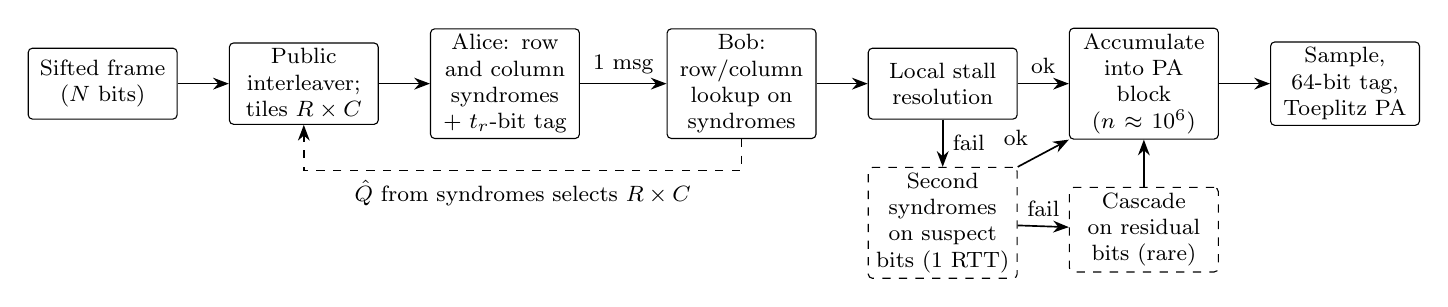
\begin{tikzpicture}[font=\footnotesize, node distance=6.5mm,
  box/.style={draw, rounded corners=1.5pt, align=center, inner sep=2pt, minimum height=9mm, text width=17.5mm},
  alt/.style={box, dashed},
  arr/.style={-{Stealth[length=2mm]}, semithick}]
\node[box] (s) {Sifted frame\\($N$ bits)};
\node[box, right=of s] (t) {Public interleaver;\\tiles $R\times C$};
\node[box, right=of t] (a) {Alice: row and column syndromes $+$ $t_r$-bit tag};
\node[box, right=11mm of a] (d) {Bob: row/column lookup on syndromes};
\node[box, right=of d] (st) {Local stall resolution};
\node[box, right=of st] (acc) {Accumulate into PA block ($n\approx10^6$)};
\node[box, right=of acc] (pa) {Sample, 64-bit tag, Toeplitz PA};
\node[alt, below=6mm of st] (f2) {Second syndromes on suspect bits (1 RTT)};
\node[alt, below=6mm of acc] (cas) {Cascade on residual bits (rare)};
\draw[arr] (s) -- (t);
\draw[arr] (t) -- (a);
\draw[arr] (a) -- node[above]{1 msg} (d);
\draw[arr] (d) -- (st);
\draw[arr] (st) -- node[above]{ok} (acc);
\draw[arr] (acc) -- (pa);
\draw[arr] (st) -- node[right]{fail} (f2);
\draw[arr] (f2) -- node[above]{fail} (cas);
\draw[arr] (f2.north east) -- node[above left, pos=0.4]{ok} (acc.south west);
\draw[arr] (cas) -- (acc);
\draw[arr, dashed] (d.south) -- ++(0,-4mm) -| node[pos=0.25, below]{$\hat Q$ from syndromes selects $R\times C$} (t.south);
\end{tikzpicture}
\caption{Reconciliation pipeline with LUCID-2D, the fallback ladder (dashed boxes) and block-level PA. Only the first message is needed when a frame decodes; the dashed arrow is the syndrome-based QBER estimate that selects the next tile shape.}
\label{fig:pipeline}
\end{figure*}

\subsection{Zero-Leakage QBER Estimation}
A block with at least one error has a non-zero syndrome difference unless the error pattern has weight at least four, so the fraction $\hat p$ of non-zero row and column differences of length $n$ gives $\hat Q=1-(1-\hat p)^{1/n}$. Bob computes it before decoding from syndromes that are already public, at no key cost, and uses it to choose the next tile shape. It does not replace the sample that bounds the phase-error rate (A4), which is taken once per PA block.

\subsection{Block-Level Verification and Privacy Amplification}\label{sec:block}
Under A5 the phase-error estimate from a sample of $k$ bits for a block of $n$ bits carries the deviation
\begin{equation}
\mu=\sqrt{\frac{(n+k)(k+1)\ln(1/\varepsilon_{\mathrm{PE}})}{2nk^{2}}},
\label{eq:mu}
\end{equation}
which is 0.45 for $n=512$, $k=64$ and $\varepsilon_{\mathrm{PE}}=10^{-10}$, far above the 11\% threshold, so per-frame PA yields no key. We reconcile per frame, accumulate verified frames into PA blocks, and extract
\begin{equation}
\ell=n\bigl[1-h(Q+\mu)\bigr]-\ell_{\mathrm{EC}}-\ell_{\mathrm{ver}}-2\log_2(1/\varepsilon_{\mathrm{PA}})
\label{eq:ell}
\end{equation}
bits. A $t_r$-bit routing tag per frame only decides on fallback, and one 64-bit tag per PA block gives the correctness guarantee. A wrong frame passes the routing tag with probability $2^{-t_r}$ and is then caught by the block tag at the cost of the block; for $t_r=24$ and at most $2^{11}$ frames per block this probability is at most $2^{-13}$. Authenticating the transcript once per block \cite{wegmancarter1981} likewise avoids spending one-time-pad key on every Cascade round.

\section{Methodology}\label{sec:method}
One Python simulator implements all schemes on the error pattern. \textit{Cascade} \cite{cascade} uses four passes with doubling blocks and back-tracking; all searches that can run in parallel do so, so its round count is a lower bound. \textit{LUCID (1-D)} uses blocks of 8--1024 bits, with whole-frame fallback at $N=512$ as in the original design and the fallback ladder elsewhere. \textit{LUCID-2D} uses tiles with $8\le R\le C\le1024$. \textit{BP-LDPC} uses a random code with variable degree three and balanced check degrees, $m=\lceil f\,h(Q)N\rceil$ syndrome bits and sum-product decoding with up to 100 iterations; failed frames are lost. Cascade and LDPC are given the true QBER.

Each parameter (block size, tile shape, Cascade first block, or $f$) is chosen on a pilot run, and the reported values come from an independent run with fresh seeds. At $N=512$ all schemes maximize $r$, as in the original study. At matched sizes, LUCID variants maximize $r$ subject to $\rho\le1.1$ (or $r/\rho$ when no parameter meets this budget), Cascade maximizes $r/\rho$, and LDPC maximizes $r$. Final runs use 2000 frames at $N=512$ and 400 (LUCID) or 100 (Cascade, LDPC) frames at $N=65536$; 95\% confidence half-widths of $r$ are at most 0.011 and 0.002, respectively. The decoder core is written in Verilog, checked cycle by cycle against a Python model of the syndrome-domain decoder with Icarus Verilog (zero mismatches in flips, convergence, scan and cycle counts over 520 random tiles of six shapes), and synthesized, placed and routed with Yosys and nextpnr \cite{shah2019}.

\section{Results}\label{sec:results}

\subsection{Validation and Reproduction}
The photon-level BB84 simulator matches $Q=e+p/4-ep/2$ to within 0.0011 at five $(e,p)$ points with $3\times10^{5}$ qubits. Table~\ref{tab:repro} reproduces the original $N=512$ comparison under frame-local accounting: secret fractions agree with the original golden model to within 0.045 and rank the schemes identically at every QBER. The 1-D hybrid trails Cascade in $r$ and lies above the unoptimized LDPC code up to 0.5\% QBER; with the block size chosen for throughput it delivers 6.0, 5.6 and 3.1 times the round-trip-limited throughput of Cascade at 0.1, 0.2 and 0.5\%, and 0.71 times at 2\%, consistent with the original study.

\begin{table}[t]
\caption{Secret Fraction $r$ and Mean Round Trips $\rho$ at $N=512$, Frame-Local Accounting}
\label{tab:repro}
\centering
\setlength{\tabcolsep}{4pt}
\begin{tabular}{@{}lcccccc@{}}
\toprule
& \multicolumn{2}{c}{Cascade} & \multicolumn{2}{c}{LUCID (1-D)} & \multicolumn{2}{c}{BP-LDPC}\\
\cmidrule(lr){2-3}\cmidrule(lr){4-5}\cmidrule(l){6-7}
QBER (\%) & $r$ & $\rho$ & $r$ & $\rho$ & $r$ & $f$\\
\midrule
0.1 & 0.828 & 6.53 & 0.818 & 1.48 & 0.750 & 6.0 \\
0.2 & 0.807 & 8.09 & 0.782 & 2.84 & 0.723 & 5.0 \\
0.5 & 0.744 & 9.70 & 0.647 & 4.18 & 0.634 & 4.0 \\
1.0 & 0.675 & 12.4 & 0.456 & 14.9 & 0.543 & 2.5 \\
2.0 & 0.551 & 19.3 & 0.378 & 24.4 & 0.422 & 2.0 \\
\bottomrule
\end{tabular}
\end{table}

\subsection{One-Round Decoding Success}
Fig.~\ref{fig:success} compares lookup-only decoding at equal frame size and row code. With 128-bit 1-D blocks a 16384-bit frame decodes with probability 0.373 at 0.1\% QBER and 0.031 at 0.2\%, and with 256-bit blocks a 65536-bit frame almost never decodes at 0.1\%. With column syndromes and stall resolution, the $128\times128$ grid decodes all 2000 frames at 0.2\% and 97.7\% at 0.5\%, and the $256\times256$ grid 99.6\% at 0.2\%. Stall resolution raises success from 0.894 to 0.977 ($128\times128$, 0.5\%) and from 0.697 to 0.859 ($256\times256$, 0.3\%).

\begin{figure}[t]
\centering
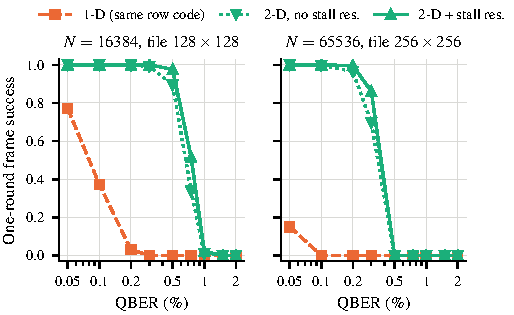
\includegraphics[width=\columnwidth]{figures/fig_success.pdf}
\caption{Probability that a frame decodes with the lookup alone, for 1-D blocks and a single square tile with the same row code.}
\label{fig:success}
\end{figure}

\subsection{Matched Frame Size}
Table~\ref{tab:matched} compares all schemes at $N=65536$ under block-level accounting, and Fig.~\ref{fig:pareto} shows every configuration of a separate sweep. At 0.1\% and 0.2\% QBER a single $256\times256$ tile reaches $r=0.919$ and $0.910$, that is 96.3\% and 98.2\% of BP-LDPC, in one round trip. Cascade attains the highest $r$ but needs 33 round trips, so LUCID-2D delivers 31 times its round-trip-limited throughput. Within one round the 1-D lookup discloses half of the key at 0.2\% ($r=0.478$ with 8-bit blocks). At 0.5\% LUCID-2D reaches 0.813 with $64\times256$ tiles at $\rho=1.12$ (94\% of BP-LDPC); at 1\% and 2\% it falls to 85\% and 52\%, and LDPC is preferable. LUCID-2D shares the one-round corner of Fig.~\ref{fig:pareto} only with LDPC, whereas Cascade and fallback-heavy 1-D configurations need tens to hundreds of round trips for comparable $r$. At $N=16384$ LUCID-2D reaches 92.9--99.4\% of BP-LDPC up to 0.5\% QBER.

\begin{table*}[t]
\caption{Secret Fraction $r$ and Mean Round Trips $\rho$ at $N=65536$, Block-Level Accounting. LUCID Parameters Were Selected for $\rho\le1.1$ on a Pilot Run Where Possible}
\label{tab:matched}
\centering
\begin{tabular}{@{}lccccccccc@{}}
\toprule
& \multicolumn{2}{c}{Cascade} & \multicolumn{2}{c}{LUCID (1-D)} & \multicolumn{3}{c}{LUCID-2D} & \multicolumn{2}{c}{BP-LDPC ($\rho=1$)}\\
\cmidrule(lr){2-3}\cmidrule(lr){4-5}\cmidrule(lr){6-8}\cmidrule(l){9-10}
QBER (\%) & $r$ & $\rho$ & $r$ & $\rho$ & tile & $r$ & $\rho$ & $r$ & $f$\\
\midrule
0.1 & 0.974 & 33.3 & 0.800 & 4.45 & $256{\times}256$ & 0.919 & 1.00 & 0.954 & 3.0 \\
0.2 & 0.953 & 33.3 & 0.478 & 5.38 & $256{\times}256$ & 0.910 & 1.00 & 0.927 & 2.5 \\
0.5 & 0.896 & 33.8 & 0.444 & 23.2 & $64{\times}256$ & 0.813 & 1.12 & 0.863 & 2.0 \\
1.0 & 0.812 & 30.8 & 0.681 & 64.8 & $32{\times}64$ & 0.642 & 1.09 & 0.757 & 2.0 \\
2.0 & 0.664 & 28.1 & 0.550 & 64.2 & $16{\times}16$ & 0.331 & 1.21 & 0.632 & 1.6 \\
\bottomrule
\end{tabular}
\end{table*}

\begin{figure}[t]
\centering
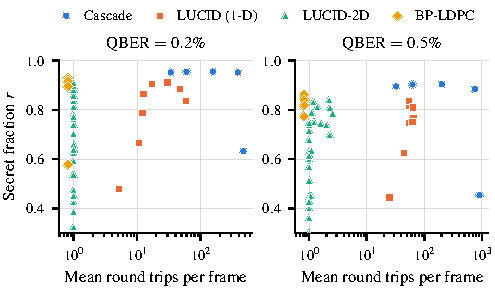
\includegraphics[width=\columnwidth]{figures/fig_pareto.pdf}
\caption{Secret fraction versus mean round trips for every configuration of a sweep at $N=65536$ (block-level accounting); LDPC points ($\rho=1$) are shifted left for visibility.}
\label{fig:pareto}
\end{figure}

\subsection{Ablation, Estimation and Finite Keys}
Without stall resolution or the second syndrome message, a $256\times256$ tile at 0.2\% falls back in 3.7\% of frames at about 20 Cascade round trips each ($\rho=1.76$); stall resolution alone gives $\rho=1.15$, the second message alone $\rho=1.03$, and both $\rho=1.00$. For $128\times128$ tiles at 0.5\% the pair reduces $\rho$ from 11.5 to 1.24. At 1\% with $64\times64$ tiles the second message alone is slightly better than both (1.85 versus 2.09), because stall guesses in tiles with many failed lines can add errors. Across all variants $r$ changes by at most 0.003.

Over equal observation windows the syndrome meter on $128\times128$ tiles has 2.7--2.9 times lower relative error than the original sampling rate of 64 bits per 512 key bits at 0.2\% QBER, and 2.2--2.4 times lower at 1\%, while disclosing nothing; a single 64-bit sample contains no error in 88\% of frames at 0.2\%. In a closed loop over 600 frames whose QBER drifts between 0.1\% and 1\%, shape selection from the syndrome estimate gives $r=0.821$ at $\rho=1.22$, matching a controller that knows the true QBER (0.821, $\rho=1.17$); a sample-driven controller reaches 0.728 because of sacrificed bits, and a fixed shape needs $\rho=14.8$.

With \eqref{eq:ell}, the leakage measured at $N=65536$ and an optimized sample size, per-frame PA on 512 bits yields no key at any QBER, whereas block-level PA at 0.2\% QBER gives finite-key fractions of 0.808 (Cascade), 0.783 (BP-LDPC) and 0.767 (LUCID-2D) at $n=2^{20}$, rising to 0.910, 0.885 and 0.868 at $n=2^{26}$; the finite-size penalty is common to all schemes.

\subsection{Burst Noise}\label{sec:burst}
With a Gilbert--Elliott channel that is error-free in the good state, flips with probability 0.25 in the bad state and keeps the mean QBER fixed, row-major tiling lets bursts of mean length 8 raise the fallback rate at 0.2\% QBER from zero to 93\% ($\rho=4.25$). The public interleaver restores it to zero for length 8 and keeps it at most 14\% (0.2\%) and 35\% (0.5\%) for length 128, with $\rho\le1.44$, at no disclosure or communication cost.

\subsection{Hardware}
Table~\ref{tab:hw} lists post-route results on a Lattice ECP5-25F. The syndrome memories map to distributed RAM, so logic grows slowly with tile size; the $256\times256$ core selected at 0.1--0.2\% QBER uses 13.1\% of the device at 61~MHz. A scan takes $R+C$ cycles, so with the 2.7 iterations measured at 0.2\% plus the final check a 65536-bit tile decodes in about 1900 cycles, 31~\textmu s, or 2.1~Gbit/s of sifted key per core---shorter than the round trip of any fibre link beyond about 3~km. For the AMD 7-series, synthesis gives 143 logic LUTs, 48 \texttt{RAM64M} and 43 flip-flops for the same core; on an iCE40 HX8K, which lacks distributed RAM, the $64\times128$ core needs 3953 logic cells at 37.8~MHz. A BP decoder for the same frame instead stores a message per edge, about 1.2~Mbit at an assumed 6-bit quantization, and ours used 7--13 iterations on average against 1.1--3.9 for LUCID-2D.

\begin{table}[t]
\caption{LUCID-2D Decoder Core After Place and Route on a Lattice ECP5 LFE5U-25F}
\label{tab:hw}
\centering
\setlength{\tabcolsep}{3.5pt}
\begin{tabular}{@{}lccccc@{}}
\toprule
Tile & LUT4 & DPRAM & FF & Logic cells used & $f_{\max}$ (MHz)\\
\midrule
$64\times128$ & 562 & 48 & 38 & 864 (3.6\%) & 84.0\\
$128\times128$ & 536 & 64 & 39 & 934 (3.8\%) & 76.2\\
$256\times256$ & 2004 & 192 & 43 & 3170 (13.1\%) & 61.1\\
\bottomrule
\end{tabular}
\end{table}

\section{Discussion and Limitations}\label{sec:discussion}
In the 0.1--0.5\% regime targeted by the original design, LUCID-2D reaches 94--98\% of the secret fraction of an oracle-tuned BP decoder in about one round trip, with 27--32 times the round-trip-limited throughput of Cascade and a hard-decision decoder that needs no QBER estimate to decode. Above about 1\% the fixed disclosure of extended-Hamming components makes it uncompetitive. The LDPC baseline is an unoptimized random code; optimized codes reach efficiencies near 1.1 at long frames \cite{elkouss2011,mao2019} and would widen its lead, although our baseline is given the true QBER and the best syndrome length. The block-level pipeline helps every scheme---Cascade rises from 0.828 at $N=512$ to 0.974 at $N=65536$ at 0.1\% QBER---and for smart-grid links, where key refresh is not latency-critical, the value of LUCID-2D lies in fewer messages and a small decoder at the edge. An optional decode cache of the original front end is omitted, since the lookup takes one cycle and caching would retain key-dependent data.

The source is ideal (A1) and the finite-key bound simplified (A5); a composable decoy-state analysis \cite{lim2014} following \cite{tsurumaru2025} is needed for deployment figures. Stall resolution, the second syndrome step and the interleaver are not yet in the RTL, the front end was not re-synthesized, and no power figures or synthesized LDPC decoder are reported. Future work covers these items and BCH components or staircase arrangements \cite{smith2012} to extend the useful QBER range.

\section{Conclusion}\label{sec:conclusion}
LUCID-BB84 reconciles BB84 keys with a one-way syndrome lookup and a verified fallback, verifying a 512-bit frame in 120~ns. Arranging frames as grids of extended-Hamming codes, decoding iteratively on syndromes, resolving stalls locally and falling back with one extra syndrome message yields a one-round reconciler within 94--98\% of BP-LDPC at 0.1--0.5\% QBER and 27--32 times the throughput of Cascade. Block-level verification and PA make the finite-key rate positive, the syndromes provide a free QBER estimate, and the verified decoder core fits in 4--13\% of a 25k-LUT FPGA. From 1\% QBER upward, one-way LDPC remains the better choice.

% balance the columns of the last page
\IEEEtriggeratref{28}
\bibliographystyle{IEEEtran}
\bibliography{refs}

\end{document}
